\chapter{Elementi di teoria dei grafi}\label{chapter:grafi}
\section{Grafi e multigrafi}
\begin{defbox}{Grafo}\index{Grafo}
    Si dice \textbf{grafo non orientato} una coppia $G=(V,R)$ dove $V$ è un insieme non vuoto ed $R$ è una relazione binaria su $V$ che gode delle proprietà:
    \begin{itemize}
        \item Antiriflessiva: $\forall u \in V \bigl((u,u) \notin R^{\#}\bigr)$
        \item Simmetrica: $\forall u,v \in V \bigl((u,v) \in R^{\#} \implies (v,u) \in R^{\#}\bigr)$
    \end{itemize}
    Dove $R^{\#}$ è il grafico della relazione $R$. Gli elementi di $V$ sono detti \textbf{vertici} del grafo; due vertici $u,v$ tali che $(u,v)\in R^{\#}$ determinano un \textbf{lato} o \textbf{arco} di $G$ che denotiamo con $\{u,v\}$. Un grafo si può rappresentare in modo del tutto equivalente come una struttura $(V,L)$ dove $L$ è l'insieme dei lati:
    \begin{equation}
        L = \{ \{x,y\} \in \mathcal{P}(V) \; | \; (x,y) \in R^{\#}\} \subseteq \mathcal{P}_{2}(V)
    \end{equation}
\end{defbox}

\begin{example}
    Consideriamo il grafo $G=(V,L)$ con cinque vertici $v_{1},v_{2},v_{3},v_{4},v_{5}$ e quattro lati:
   \begin{displaymath}
    \begin{array}{llll}
        l_{1}= \{v_{1},v_{2}\}, & l_{2} = \{v_{2},v_{3}\}, & l_{3}\{v_{3},v_{4}\}, & l_{4}=\{v_{2},v_{4}\}
    \end{array}
   \end{displaymath}
    Allora $G$ ha la seguente rappresentazione:
    \begin{center}
        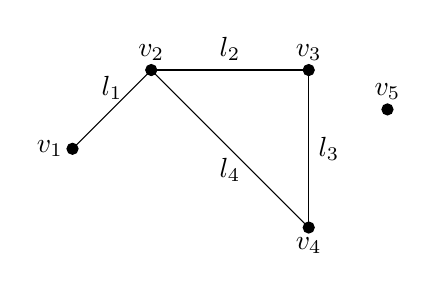
\begin{tikzpicture}
            \filldraw[black] (0,0) circle (2pt) node[anchor=east]{$v_{1}$};
            \filldraw[black] (1,1) circle (2pt) node[anchor=south]{$v_{2}$};
            \filldraw[black] (3,1) circle (2pt) node[anchor=south]{$v_{3}$};
            \filldraw[black] (3,-1) circle (2pt) node[anchor=north]{$v_{4}$};
            \filldraw[black] (4,.5) circle (2pt) node[anchor=south]{$v_{5}$};
            \draw[-] (0,0)to node[above,midway]{$l_{1}$} (1,1);
            \draw[-] (1,1) to node[above,midway]{$l_{2}$}(3,1);
            \draw[-] (3,1) to node[right,midway]{$l_{3}$}(3,-1);
            \draw[-] (3,-1) to node[below,midway]{$l_{4}$}(1,1);
        \end{tikzpicture}
    \captionof{figure}{Esempio di grafo non orientato}\label{fig:grafo}
    \end{center}
\end{example}

\begin{defbox}{Adiacenza}
    Due vertici $u,u' \in V$ si dicono \textbf{adiacenti} se $\{u,u'\} \in L$. Diremo allora che il lato $l=\{u,u'\}$ \textbf{collega} $u$ e $u'$.
\end{defbox}

\begin{osservation}
	Possiamo dunque intendere un grafo come una sorta di carta geografica in cui i vertici rappresentano i centri abitati e i lati le strade che li congiungono. La proprietà antiriflessiva ci dice che non ci sono strade che, partendo da un paese, vi ritornano senza tappe intermedie; la proprietà simmetrica che ogni strada si percorre a doppio senso.
\end{osservation}

Se aboliamo le proprietà antiriflessiva e simmetrica, e quindi ammettiamo che esistano strade che partono e arrivano allo stesso vertice, e che ogni strada tra due vertici sia a senso unico, otteniamo il concetto di \textbf{grafo orientato} (o \textbf{grafo diretto}, o \textbf{disgrafo}).

\begin{center}
	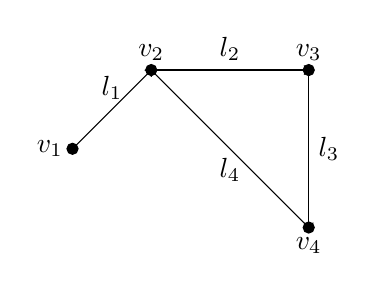
\begin{tikzpicture}
		\filldraw[black] (0,0) circle (2pt) node[anchor=east]{$v_{1}$};
		\filldraw[black] (1,1) circle (2pt) node[anchor=south]{$v_{2}$};
		\filldraw[black] (3,1) circle (2pt) node[anchor=south]{$v_{3}$};
		\filldraw[black] (3,-1) circle (2pt) node[anchor=north]{$v_{4}$};
		\draw[->] (0,0)to node[above,midway]{$l_{1}$} (1,1);
		\draw[->] (1,1) to node[above,midway]{$l_{2}$}(3,1);
		\draw[->] (3,1) to node[right,midway]{$l_{3}$}(3,-1);
		\draw[->] (3,-1) to node[below,midway]{$l_{4}$}(1,1);
	\end{tikzpicture}
\captionof{figure}{Esempio di grafo orientato}
\end{center}

\begin{defbox}{Incidenza}
    Due lati $l,l' \in L$ si dicono \textbf{incidenti} nel vertice $v$ o \textbf{consecutivi} se $\{v\} = l \cap l'$, cioè se $v$ è l'unico estremo comune di $l$ ed $l'$.
\end{defbox}
\begin{example}
	Osservando il grado in Figura \ref{fig:grafo} abbiamo che i lati $l_{1}$ e $l_{2}$ sono incidenti in $v_{2}$.
\end{example}
\begin{defbox}{Vertici isolati}
    Un vertice si dice \textbf{isolato} se non ci sono lati di $L$ incidenti in $v$.
\end{defbox}
\begin{example}
	Il vertice $v_{5}$ del grafo in Figura \ref{fig:grafo} è isolato.
\end{example}
\begin{defbox}{Grafo finito}
    Un grafo si dice \textbf{finito} se tale è l'insieme $V$ dei suoi vertici.
\end{defbox}
\begin{example}
	Il grafo in Figura \ref{fig:grafo} è finito.
\end{example}

\begin{defbox}{Grado}
    Il \textbf{grado} di un vertice $v$ è il numero di lati incidenti in $v$. Lo indichiamo con $deg(v)$. Un vertice isolato ha grado zero. Un vertice $v \in V$ si dice \textbf{pari} o \textbf{dispari} a seconda che $deg(v)$ sia pari o dispari. Un grafo avente tutti i vertici dello stesso grado $d$ si dice \textbf{regolare} di grado $d$.
\end{defbox}
\begin{example}
	Nel grafo in Figura \ref{fig:grafo} il vertice $v_{2}$ ha grado 3 e si scriverà $deg(v_{2})=3$ e risulta essere un verdice dispari.
\end{example}
\begin{defbox}{Grafo completo}
    Il grafo $G=(V,L)$ si dice \textbf{completo} se tutti i suoi vertici sono a due a due adiacenti, cioè, se per ogni scelta di $u,v \in V$ con $u \neq v$ $\{u,v\} \in L$.
\end{defbox}

\begin{example}
    Proponiamo alcuni esempi di grafi completi, rispettivamente con 1, 2, 3, 4 vertici. Li denotiamo, nell'ordine, $K_{1},\ K_{2},\ K_{3},\ K_{4}$.
    \begin{center}
    \begin{minipage}{.2\textwidth}
        \centering
        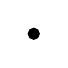
\begin{tikzpicture}
            \filldraw[black](0,0) circle (2pt);
        \end{tikzpicture}

        $K_{1}$
    \end{minipage}
    \begin{minipage}{.2\textwidth}
        \centering
        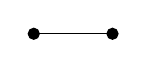
\begin{tikzpicture}
            \filldraw[black] (0,0) circle (2pt);
            \filldraw[black] (1,0) circle (2pt);
            \draw[-](0,0)--(1,0);
        \end{tikzpicture}

        $K_{2}$
    \end{minipage}
    \begin{minipage}{.2\textwidth}
        \centering
        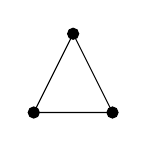
\begin{tikzpicture}
            \filldraw[black] (0,0) circle (2pt);
            \filldraw[black] (.5,1) circle (2pt);
            \filldraw[black] (1,0) circle (2pt);
            \draw[-](0,0)--(1,0) --(.5,1)--(0,0);
        \end{tikzpicture}

        $K_{3}$
    \end{minipage}
    \begin{minipage}{.2\textwidth}
        \centering
        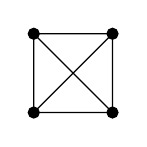
\begin{tikzpicture}
            \filldraw[black] (0,0) circle (2pt);
            \filldraw[black] (1,1) circle (2pt);
            \filldraw[black] (0,1) circle (2pt);
            \filldraw[black] (1,0) circle (2pt);
            \draw[-](0,0)--(1,0) --(1,1)--(0,1)--(0,0)--(1,1);
            \draw[-](0,1)--(1,0);
        \end{tikzpicture}

        $K_{4}$
    \end{minipage}
\end{center}	Per ogni intero positivo $n$ la struttura di un grafo completo di $n$ vertici è determinata. Ci sono appunto $n$ vertici e ogni coppia di vertici distinti è collegata da un lato. In genere, per ogni intero positivo $n$, l'``unico'' grafo completo con $n$ vertici è indicato con $K_{n}$. Si noti poi, che ogni grafo $G$ è sottografo di un opportuno grafo completo.
\end{example}

\begin{osservation}
	Ovviamente ogni grafo completo risulta un grafo regolare ma non vale il viceversa. Si consideri il seguente grafo regolare di grado 2:
	\begin{center}
		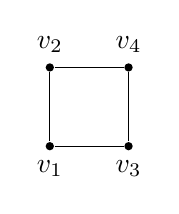
\begin{tikzpicture}
			\node[circle,fill=black,inner sep=0pt,minimum size=3pt,label=below:{$v_{1}$}](a) at (0,0){};
			\node[circle,fill=black,inner sep=0pt,minimum size=3pt,label=above:{$v_{2}$}](b) at (0,1){};
			\node[circle,fill=black,inner sep=0pt,minimum size=3pt,label=below:{$v_{3}$}](c) at (1,0){};
			\node[circle,fill=black,inner sep=0pt,minimum size=3pt,label=above:{$v_{4}$}](d) at (1,1){};
			\draw[black,thin](a)--(b);
			\draw[black,thin](c)--(d);
			\draw[black,thin](b)--(d);
			\draw[black,thin](a)--(c);
		\end{tikzpicture}
	\end{center}
Chiaramente non è completo in quanto non esiste un lato che colleghi $v_{2}$ e $v_{3}$ e $v_{1}$ con $v_{4}$. 
\end{osservation}

\begin{propbox}
	Un grafo $G=(V,L)$ è completo se, e solo se, $L=\mathcal{P}_{2}(V)$. Ovvero se per ogni intero positivo $n$, il grafo $K_{n}$ ha esattamente:
\begin{displaymath}
    |\mathcal{P}_{2}(V)| = \binom{n}{2} = \frac{n(n-1)}{2}
\end{displaymath}
lati.
\end{propbox}
\begin{proof}
	\begin{itemize}
		\item[$\implies$] Se $G=(V,L)$ è un grafo completo allora tutti i vertici sono in relazione $R$ tra di loro, ciò significa che $R$ è totale e che per ogni $u,v \in V$ esiste un lato $l=\{u,v\} \in L$. Si ha allora $L=\mathcal{P}_{2}(V)$ e vale:
		\begin{align*}
			|L| = |\mathcal{P}_{2}(V)| &= \binom{n}{2} \\
			&= \frac{n!}{2 \cdot (n-2)!} \\
			&= \frac{n (n-1)!}{2 \cdot (n-2)(n-3)!} \\
			&= \frac{n (n-1)(n-2)\cdot \ldots 1}{2(n-2)(n-2)(n-4)\cdot \ldots \cdot 1}\\
			&= \frac{n(n-1)}{2}
		\end{align*}
	\item[$\impliedby$] Ovvio per le osservazioni fatte in precedenza.
	\end{itemize}
\end{proof}
\begin{corolbox}
	Un grafo $G=(V,L)$ con $n$ vertici ha al più $\binom{n}{2}$ lati, che risulta essere un \textit{limite superiore} al numero possibile di vertici in un grafo finito.
\end{corolbox}

\begin{defbox}{Grafo planare}
    Un grafo $G=(V,L)$ si dice \textbf{planare} se può essere rappresentato senza che i lati si intersechino tra loro.
\end{defbox}

\begin{example}
    Si ha che il grafo mostrato a sinistra è planare mentre quello a destra non lo è:
    \begin{center}
        \begin{minipage}{.2\textwidth}
            \centering
            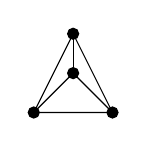
\begin{tikzpicture}
            \filldraw[black] (0,0) circle (2pt);
            \filldraw[black] (.5,.5) circle (2pt);
            \filldraw[black] (.5,1) circle (2pt);
            \filldraw[black] (1,0) circle (2pt);
            \draw[-](0,0)--(1,0) --(.5,1)--(0,0);
            \draw[-](0,0)--(.5,.5);
            \draw[-](.5,.5)--(.5,1);
            \draw[-](.5,.5)--(1,0);
            \end{tikzpicture}
        \end{minipage}
        \hfil
        \begin{minipage}{.2\textwidth}
            \centering
            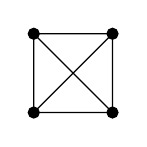
\begin{tikzpicture}
                \filldraw[black] (0,0) circle (2pt);
                \filldraw[black] (1,1) circle (2pt);
                \filldraw[black] (0,1) circle (2pt);
                \filldraw[black] (1,0) circle (2pt);
                \draw[-](0,0)--(1,0) --(1,1)--(0,1)--(0,0)--(1,1);
                \draw[-](0,1)--(1,0);
            \end{tikzpicture}
        \end{minipage}
    \end{center}
\end{example}


\subsection{Isomorfismi tra grafi}
\dfn{Isomorfismo}{
    Due grafi $G_{1}=(V_{1},L_{1})$, $G_{2}=(V_{2},L_{2})$ si dicono \textbf{isomorfi} se esiste una biiezione $f: V_{1} \rightarrow V_{2}$ tale che, per ogni scelta di $u,v \in V_{1}$ si ha:
    \begin{displaymath}
        \{u,v\} \in L_{1} \iff \{f(u),f(v)\} \in L_{2}
    \end{displaymath}
    ed $f$ si dice \textbf{isomorfismo} di $G_{1}$ su $G_{2}$.
}

\begin{osservation}
	Chiaramente, se un diagramma rappresenta un grafo $G$, lo stesso diagramma rappresenta ogni grafo isomorfo a $G$.
\end{osservation}

\begin{defbox}{Sottografo}
	Se $G=(V,L)$ è un grafo, $V'$ è un sottoinsieme di $V$ ed $L'$ è un sottoinsieme di $L$ tale che per ogni lato $l=\{u,v\} \in L'$ i suoi estremi $u,v$ stanno in $V'$, allora $G'=(V',L')$ è un grafo, detto \textbf{sottografo} di $G$. 
\end{defbox}
\subsection{Multigrafi}

\begin{defbox}{Multigrafo}
	Un \textbf{multigrafo semplice} è una terna $(V,L,\varphi)$ in cui:
	\begin{itemize}
		\item $V$ è un insieme non vuoto di vertici;
		\item $L$ è un insieme di lati;
		\item $\varphi$ è una funzione da $L$ in $\mathcal{P}_{2}(V)$ detta \textbf{funzione di incidenza}.
	\end{itemize}
\end{defbox}

\begin{osservation}
	I grafi non sono altro che multigrafi in cui $\varphi$ risulta iniettiva.
\end{osservation}

Infatti rispetto alla nozione di grafo, abbiamo l'ovvia complicazione tecnica che due vertici distinti $u$ e $v$ possono essere collegati da più di un lato; la notazione $\{u, v\}$ non basta allora a identificare tutti i lati tra $u$ e $v$, e si deve ricorrere alla funzione di incidenza $\varphi$ per chiarire la situazione. Infatti l'applicazione $\varphi$ associa ad ogni lato $l \in L$  l'insieme $\{u, v\}$ dei suoi estremi. In un multigrafo non si richiede che $\varphi$ sia iniettiva, e quindi $\varphi$ può associare la stessa coppia di estremi a più lati distinti: si parla allora di lati \textbf{multipli} tra gli stessi estremi.

\begin{example}
	Si consideri il multigrafo $G=(V,L,\varphi)$ dove $V = \{v_{1},v_{2},v_{3},v_{4}\}$, $L=\{l_{1},l_{2},l_{3}\}$, $\varphi(l_{1})=\{v_{1},v_{2}\}$, $\varphi(l_{2})=\varphi(l_{3}) = \{v_{2},v_{3}\}$. I lati multipli sono $l_{2}$ ed $l_{3}$. Si ha quindi la seguente rappresentazione grafica:
	\begin{center}
		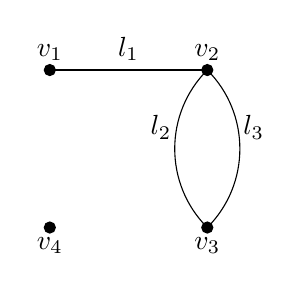
\begin{tikzpicture}
			\filldraw[black] (0,0) circle (2pt) node[anchor=north]{$v_{4}$};
			\filldraw[black] (2,2) circle (2pt)node[anchor=south]{$v_{2}$};
			\filldraw[black] (0,2) circle (2pt) node[anchor=south]{$v_{1}$};
			\filldraw[black] (2,0) circle (2pt) node[anchor=north]{$v_{3}$};
			\draw[-] (0,2)--node[midway,above]{$l_{1}$}(2,2);
			\draw[-,bend angle=45, bend right] (2,2) to node[above,xshift=-5pt]{$l_{2}$} (2,0);
			\draw[-,bend angle=45,bend left] (2,2) to node[above,xshift=5pt]{$l_{3}$} (2,0);
		\end{tikzpicture}
	\end{center}
\end{example}


\begin{osservation}
	    La nozione di isomorfismo ha il suo opportuno adattamento tra i multigrafi. Due multigrafi $G_{1}=(V_{1},L_{1},\varphi)$ e $G_{2}=(V_{2},L_{2},\psi)$ si dicono \textbf{isomorfi} se esistono due biezioni: $f: V_{1} \rightarrow V_{2}$ e $g: V_{2} \rightarrow V_{1}$ tali che, per ogni scelta di $l \in L_{1}$ e $u,v \in V_{1}$ si ha:
    \begin{displaymath}
        \varphi(l) = \{u,v\} \iff \psi(g(l))= \{f(u),f(v)\}
    \end{displaymath}
\end{osservation}


\begin{teorbox}
	    Sia $G=(V,L,\varphi)$ un multigrafo finito. Allora:
    \begin{displaymath}
        \sum_{v \in V} deg(v) = 2 |L|
    \end{displaymath}
\end{teorbox}

\begin{proof}
	Sia $S=\{(v,l) \in V \times L \; | \; \text{$v$ è un estremo di $l$}\}$. Rappresentiamo $S$ mediante una tabella in cui poniamo delle crocette se, e solo se, $v_{i}$ è un estremo di $l_{j}$:
\begin{center}
    \begin{tblr}{hlines,vlines,row{1}={primary!80!white},column{1}={primary!80!white},cells={mode=math}}
        & l_{1} & l_{2} & l_{3} & \dots & l_{r} \\
        v_{1} &  \times & & &\times &\\
        v_{2} & & \times& & &\\
        v_{3} & \times & &\times & &\times \\
        \vdots & & & \times & \times &\\
        v_{r} & &\times & & &\times
    \end{tblr}
\end{center}
Dato che ogni lato ha sempre due estremi, ogni colonna avrà sempre due crocette. Quindi per ogni lato del multigrafo corrispondono due elementi dell'insieme $S$: $|S|=2L$. Analogamente, contando per righe, il numero di crocette presente su ogni riga denoterà il numero di lati incidenti sul vertice corrispondente alla riga, ovvero il grado del vertice. Quindi possiamo dire con certezza che $S = \sum_{v \in V} deg(v)$ concludendo così la dimostrazione.
\end{proof} 


\begin{osservation}
	    Come conseguenza del teorema, i vertici pari di un multigrafo possono essere di un numero arbitrario mentre quelli dispari devono essere in numero pari. Infatti, denotato con $V_{p}$ e $V_{d}$ gli insiemi dei vertici pari e dispari di $V$ si ha:
    \begin{displaymath}
        \sum_{v \in V} deg(v) = \sum_{v \in V_{p}} deg(v) + \sum_{v \in V_{d}} deg(v)
    \end{displaymath}
    Ovviamente, $\sum_{v \in V_{p}} deg(v)$ è pari, pertanto anche $\sum_{v \in V_{d}} deg(v) = \sum_{v \in V} deg(v) - \sum_{v \in V_{p}} deg(v)$ è un numero pari, perché differenza di numeri pari. Ma $\sum_{v \in V_{d}} deg(v)$ è la somma di addendi dispari, e dunque è pari se e solo se il numero dei suoi addendi, e cioè dei vertici dispari, è pari.
\end{osservation}

\section{Cammini e circuiti in un grafo}

\dfn{Cammino}{
    Siano $G=(V,L)$ un grafo, $u,w \in V$. Si dice \textbf{cammino}\index{Cammino} di $G$ tra $u$ e $w$ una sequenza finita $\alpha = (l_{1},l_{2}, \ldots, l_{m})$ di lati di $L$ a due a due distinti tali che, per ogni $i< m$, $l_{i+1}$ è consecutivo ad $l_{i}$. Se un cammino passa per tutti i lati del grafo allora verrà chiamato \textbf{cammino euleriano}\index{Cammino!Euleriano}.
}
\dfn{Circuito}{\index{Circuito}
    Un \textbf{circuito} o \textbf{ciclo} è un cammino da un vertice a se stesso. Se un cammino passa per ogni lato di un multigrafo una ed una sola volta allora viene chiamato \textbf{circuito euleriano}\index{Circuito!Euleriano}. Un grafo che contiene un ciclo è detto \textbf{ciclico}.
}

\dfn{Grafo connesso}{
    Un grafo $G=(V,L)$ si dice \textbf{connesso} se per ogni coppia di vertici distinti $u,v \in V$ esiste un cammino tra $u$ e $v$.
}

\begin{teorbox}[di Eulero]
	    Sia $G$ un multigrafo finito senza vertici isolati. Allora $G$ ha un circuito euleriano se e solo se $G$ è connesso e tutti i suoi vertici sono pari.
\end{teorbox}

\begin{example}
	Si osservi il seguente grafo orientato finito, senza vertici isolati, in cui ogni vertice ha grado pari:
	\begin{center}
		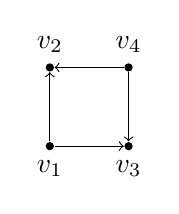
\begin{tikzpicture}
			\node[circle,fill=black,inner sep=0pt,minimum size=3pt,label=below:{$v_{1}$}](a) at (0,0){};
			\node[circle,fill=black,inner sep=0pt,minimum size=3pt,label=above:{$v_{2}$}](b) at (0,1){};
			\node[circle,fill=black,inner sep=0pt,minimum size=3pt,label=below:{$v_{3}$}](c) at (1,0){};
			\node[circle,fill=black,inner sep=0pt,minimum size=3pt,label=above:{$v_{4}$}](d) at (1,1){};
			\draw[black,thin,->](a)--(b);
			\draw[black,thin,->](d)--(c);
			\draw[black,thin,->](d)--(b);
			\draw[black,thin,->](a)--(c);
		\end{tikzpicture}
	\end{center}
	È evidente che tale grafo non è connesso in quanto non esiste un cammino tra i vertici $v_{1}$ e $v_{4}$. Di conseguenza si può osservare che non esiste un circuito euleriano per nessuno dei quattro vertici.
\end{example}

\begin{corolbox}
	Sia $G$ un multigrafo finito privo di vertici isolati. Il multigrafo $G$ ha un cammino euleriano se e solo se è connesso ha zero o due vertici dispari.
\end{corolbox}

\begin{osservation}
	La relazione di connessione, o di \textit{raggiungibilità}, è una relazione di equivalenza in quanto risulta essere riflessiva, simmetrica e transitiva. Per questo motivo possiamo considerare l'insieme quoziente di $V$ rispetto a tale equivalenza. Gli elementi di tale quoziente vengono chiamati \textbf{componenti connesse} e sono formati da vertici connessi e dai lati che formano i cammini che li connettono.
\end{osservation}


\section{Foreste ed alberi}

\dfn{Foresta ed alberi}{
    Chiamiamo \textbf{foresta} un grafo senza circuiti (\textbf{grafo aciclico}), e \textbf{albero} un grafo connesso senza circuiti (\textit{grafo aciclico connesso}).
}

Il collegamento tra i due nomi (alberi e foreste) è chiaro: infatti, la assenza di circuiti si trasmette ovviamente ai sottografi, ed è dunque facile osservare che le componenti connesse di una foresta sono, appunto, alberi.


\begin{teorbox}
	    Un grafo finito $G=(V,L)$ è una foresta se, e solo se, per ogni coppia di vertici $(a,b)$ con $a \neq b$ esiste al più un cammino. Un grafo finito è un albero se, per tale coppia esiste esattamente un cammino.
\end{teorbox}

\begin{proof}
	Siano $a,b \in V$. Siccole $G$ è connesso, c'è almeno un cammino tra $a$ e $b$. Ammettiamo che ce ne siano due, $\alpha$ e $\alpha'$ rispettivamente. Se $\alpha$ e $\alpha'$ non hanno lati comuni, il cammino che segue $\alpha$ da $a$ a $b$ e poi da $b$ ad $a$ lungo $\alpha'$ è un circuito di $G$ e questo è assurdo. Anche nel caso in cui $\alpha$ e $\alpha'$ abbiano un lato in comune si costruisce un circuito in $G$ e si cade dunque in contraddizione. Quindi esiste un unico cammino lungo tale grafo connesso che risulta quindi essere un albero.
\end{proof}

\subsection{Rappresentazione radiale di un albero}

È possibile rappresentare un albero $G=(V,L)$ selezionandone un vertice, che chiameremo \textbf{radice} e disponendo poi gli altri punti di $V$ nelle ramificazioni che si dipartono dalla radice. Tale rappresentazione prende il nome di \textbf{rappresentazione radiale} di $G$.

\begin{osservation}
	Una foresta finita è necessariamente un grafo planare.
\end{osservation}

\begin{example}
    Si consideri la seguente rappresentazione generica del grafo $G$:
    \begin{center}
    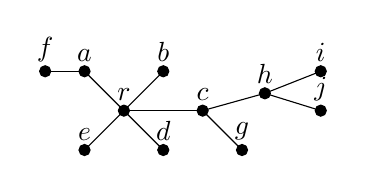
\begin{tikzpicture}
        \filldraw[black] (.5,.5) circle(2pt) node[anchor=south]{$a$};
        \filldraw[black] (1.5,.5) circle(2pt) node[anchor=south]{$b$};
        \filldraw[black] (1.5,-.5) circle(2pt) node[anchor=south]{$d$};
        \filldraw[black] (.5,-.5) circle(2pt) node[anchor=south]{$e$};
        \filldraw[black] (0,.5) circle(2pt) node[anchor=south]{$f$};
        \filldraw[black] (2,0) circle(2pt) node[anchor=south]{$c$};
        \filldraw[black] (2.5,-.5) circle(2pt) node[anchor=south]{$g$};
        \filldraw[black] (2.79,.22) circle(2pt) node[anchor=south]{$h$};
        \filldraw[black] (3.5,.5) circle(2pt) node[anchor=south]{$i$};
        \filldraw[black] (1,0) circle(2pt) node[anchor=south]{$r$};
        \filldraw[black] (3.5,0) circle(2pt) node[anchor=south]{$j$};
        \draw[-](.5,.5)--(0,.5);
        \draw[-](.5,.5)--(1,0);
        \draw[-](1,0)--(.5,-.5);
        \draw[-](1,0)--(1.5,.5);
        \draw[-](1,0)--(1.5,-.5);
        \draw[-](1,0)--(2,0);
        \draw[-](2,0)--(2.79,.22);
        \draw[-](2,0)--(2.5,-.5);
        \draw[-](2.79,.22)--(3.5,.5);
        \draw[-](2.79,.22)--(3.5,0);
    \end{tikzpicture}
\end{center}

Selezionato il vertice $r$ come radice dell'albero, si ottiene la seguente rappresentazione radiale:
\begin{center}
    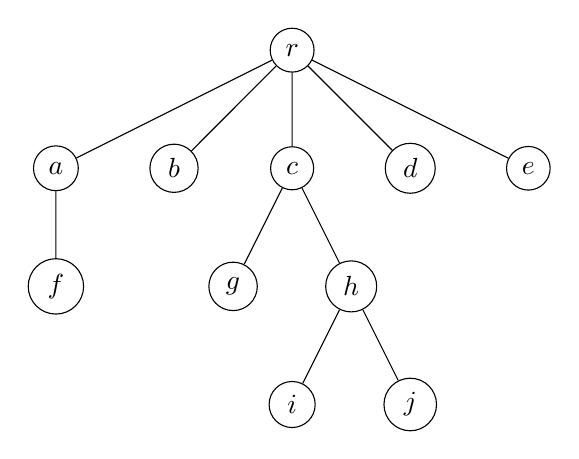
\begin{tikzpicture}
        [every node/.style={circle,draw,minimum size=2pt}]
        \node{$r$}
        child{
            node{$a$}
            child{
                node{$f$}
            }
        }
        child{
            node{$b$}
        }
        child{
            node{$c$}
            child{
                node{$g$}
            }
            child{
                node{$h$}
                child{
                    node{$i$}
                }
                child{
                    node{$j$}
                }
            }
        }
        child{
            node{$d$}
        }
        child{
            node{$e$}
        };
    \end{tikzpicture}
\end{center}
\end{example}


\begin{defbox}{Foglia}
	Se un albero ha almeno due vertici in rappresentazione radiale, chiameremo \textbf{foglie} i vertici a distanza massima dalla radice. Tali vertici avranno grado pari ad uno in quanto esiste un solo lato incidente su tali vertici, ovvero il lato proveniente dal vertice ``padre''.
\end{defbox}


\begin{lemmabox}
	    Sia $T=(V,L)$ un albero e sia $v \in V$ tale che $deg(v) = 1$. Si ha che $v$ è una foglia. Sia $l \in L$ tale che $v$ è un estremo di $l$. Allora $T'=(V\setminus \{v\}, L \setminus \{l\})$ è ancora un albero.
\end{lemmabox}


\begin{proof}
	 Per ogni $a,b \in T'$ si ha sicuramente che $a \neq v$ e $b \neq v$ e quindi il cammino tra $a$ e $b$ non è $l$ perché ogni vertice che non sia un estremo di un cammino ha sempre grado maggiore o uguale a due. 
\end{proof}


\begin{propbox}
	    Se $G = (V,L)$ è un albero finito con $n$ vertici allora $G$ ha esattamente $n-1$ lati. Vale cioè la seguente uguaglianza:
    \begin{displaymath}
        |G| = |L|+1
    \end{displaymath}
\end{propbox}

\begin{proof}
	Sia $G = (V, L)$ un albero finito. Sappiamo che G è privo di circuiti, dobbiamo provare che, se $G$ ha $n$ vertici, allora $G$ ha $n-1$ lati. Si procede per induzione su $n$. Il caso $n = 1$ è banale: un albero con 1 solo vertice non ha né lati né circuiti. Assumiamo ora la tesi vera per $n$ e proviamola per $n + 1$. Sia
quindi $G = (V, L)$ un albero con $n + 1 \geq 2 $ vertici. Per il lemma precedente
$G$ ha almeno una foglia (in realtà almeno due foglie), cioè almeno un vertice
$v$ di grado 1. Questo significa che in $G$ c'è un unico lato $l$ che ha estremo $v$.
Se eliminiamo dall'albero $G$ il vertice $v$ e il lato $l$ otteniamo un grafo $G_{0}$ che
è ancora connesso e privo di circuiti, dunque è un albero. Ma $G_{0}$ ha $n$ vertici,
quindi per l'ipotesi induttiva $G_{0}$ ha $n-1$ lati. Di conseguenza $G$ ha $n$ lati: gli
$n-1$ di $G_{0}$ più 1.
\end{proof}

\subsection{Sottoalberi massimali}

\dfn{Sottografo massimale}{
Sia $G=(V,L,\varphi)$ un multigrafo finito. Un \textbf{sottoalbero massimale} di $G$ è un sottografo $G$ con insieme di vertici $V$ che sia un albero.
}

Si dimostra facilmente che se elimino un lato da un circuito i vertici $v \in V$ restano ancora tutti connessi. Infatti:

\begin{propbox}
	Sia $G=(V,L, \varphi)$ un multigrafo connesso. Sia $l_{0} \in L$ tale che $l$ faccia parte di un circuito in $G$. Allora il sottografo $G'=(V,L',\varphi')$ con $L'=L \setminus \{l_{0}\}$ è ancora connesso.
\end{propbox}

\begin{proof}
	 Siano $a,b \in G$. Se $a,b$ sono connessi da un circuito, allora esistono almeno due cammini diversi da $a$ a $b$ siano essi $\nu$ e $\mu$. Se $l_{0}$ si trova nel cammino $\nu$ allora $a$ e $b$ sono connessi da $\mu$ in $G'$, o viceversa.
\end{proof}

\begin{teorbox}[Teorema conclusivo]
Sia $G=(V,L,\varphi)$ un multigrafo finito con esattamente $k$ componenti connesse. Allora:
\begin{enumerate}
    \item Se $G$ è connesso allora $|L| \geq |V|-1$
    \item $|L| \geq |V|-k$
    \item $|L| = |V|-k$ se, e solo se, $G$ è una foresta
    \item Sono equivalenti: \begin{enumerate}
        \item $G$ è un albero
        \item $G$ è connesso e $|V|=|L|+1$
        \item $G$ è una foresta e $|V|=|L|+1$
    \end{enumerate}
\end{enumerate}
\end{teorbox}
\begin{proof}
	\begin{enumerate}
    \item Se $G$ è connesso allora $G$ ha un sottoalbero massimale $(V,L')$ con $L' \subseteq L$. Allora $|V|=|L'|+1$, quindi $|L'|=|V|-1$ e dato che $|L'|\leq |L| \implies |L| \geq |V|-1$, ovvero vale $|V|=|L|+1 \iff |L|=|L'| \iff L=L'$.
    \item Siano $(V_{1},L_{1},\varphi_{1})$, $(V_{2},L_{2},\varphi_{2})$,...,$(V_{k},L_{k},\varphi_{k})$ le componenti connesse di $G$, per ogni $i \in \{1,...,k\}$ si ha $|L_{i}| \geq |V_{i}|-1$ per la $(1)$. Allora, essendo:$|L|=\sum_{i=1}^{k} |L_{i}|$, $|V|=\sum_{i=1}^{k} |V_{i}|$e $\sum_{i=1}^{k} -1 = -k$ si ha: $|L| \geq |V|-k$.
    \item Se per ogni $i \in \{1,...,k\}$ $|L_{i}| = |V_{i}|-1$ allora $|L|=|V|-k$ per la $(2)$, inoltre $G_{i}=(V_{i},L_{i})$ è un albero. Quindi $G$ è una foresta.
    \item $(b) \implies (a)$ per la $(1)$. Mentre $(a) \implies (b)$ è stato già dimostrato.

    $(a) \implies (c)$: se $G$ è un albero, allora $G$ è anche una foresta. Inoltre, per la $(3)$ si ha $|V|=|L|+k$, dove $k$ sono le componenti connesse in $G$. Essendo $G$ un albero deve essere $k=1$.

    $(c) \implies (a)$: per la $(3)$ $G$ è una foresta con $k=1$ componenti connesse, quindi $G$ è un albero.
\end{enumerate}
\end{proof}
\newpage
\section{Esercizi svolti}
	\begin{exsbox}
		Vero o falso? Le foreste finite sono grafi planari.
	\end{exsbox}
	\begin{exsbox}
		Dimostrare che se due grafi $G$ e $G′$ sono isomorfi, anche il grafo complementare di $G$ ed il grafo complementare di $G′$ sono isomorfi tra loro.
	\end{exsbox}
	\begin{exsbox}
		Un grafo $G$ ha 7 lati e 8 vertici, sette dei quali hanno grado 1. Qual è il grado dell’ottavo vertice?
		Disegnare un grafo con queste proprietà. Esistono due siffatti grafi tra loro non isomorfi? Un tale grafo è un albero? Esistono grafi con 7 lati e 8 vertici che non siano alberi?
	\end{exsbox}
	\begin{exsbox}
		Esiste un grafo con cinque lati e almeno tre vertici di grado 4?
	\end{exsbox}
	\begin{exsbox}
		Un grafo connesso $G$ ha 9 vertici. Di questi, almeno 6 sono pari. Questi dati sono sufficienti per stabilire se $G$ ha cammini euleriani?
	\end{exsbox}
	\begin{exsbox}
		Si considerino i grafi $G=(V,L)$ che verificano la proprietà $\Phi$:``$|V|=6=|L|$ ed esistono in $G$ (almeno) un vertice di grado 4 ed (almeno) tre vertici di grado 2''.
		\begin{enumerate}
			\item Se un grafo $G$ verifica $\Phi$, quali possono essere i gradi dei suoi vertici?
			\item Disegnare, se possibile, un grafo che verifichi $\Phi$;
			\item Disegnare, a meno di isomorfismi, tutti i grafi che verificano $\Phi$.
		\end{enumerate}
	\end{exsbox}
	\begin{exsbox}
		Stabilire per quali interi positivi $n$ il grafo completo su $n$ vertici abbia cammini euleriani e per quali abbia circuiti euleriani.
	\end{exsbox}